\documentclass[a4paper, 10pt]{scrartcl}
\usepackage[utf8]{inputenc}
\usepackage[ngerman]{babel}
\usepackage[T1]{fontenc}
\usepackage{helvet}
\usepackage{hyperref}
\usepackage{natbib}
\usepackage{graphicx}
\makeatletter
\renewcommand\paragraph{\@startsection{paragraph}{4}{\z@}%
			{-2.5ex \@plus -1ex\@minus -.25ex}%
			{1.25ex \@plus .25ex}%
			{\normalfont\normalsize\bfseries}}
\makeatother
\setcounter{secnumdepth}{4}
\setcounter{tocdepth}{4}			

\bibliographystyle{unsrt}
\begin{document}



\section{Die klassische bzw. statische Softwareentwicklung}
\subsection{Definition}
\begin{center}
\large{Klassische bzw. statische Softwareentwicklung ist eine Form der Softwareentwicklung bei welcher ein \glqq Software Development Life Cycle (SDLC)\grqq{} nach festem Ablaufplan umgestzt wird.\citep{stoica}} 
\end{center}
\subsection{Funktionsweise der klassichen bzw. statischen Softwareentwicklung}
Die klassiche Softwareentwicklung funktioniert nach dem Prinzip des SDLC. Dieser besteht aus 6 Phasen, welche alle nacheinander vom Entwicklungsteam abgearbeitet werden müssen.\citep{stoica} (siehe Abbildung 1)
\subsubsection{Analyse und Planung}
Die erste Phase dieses SDLC besteht aus der Analyse und Planung des Projektes. Sie ist gleichzeitig auch der wichtigste Entwicklungsabschnitt. Deshalb sollte dieser Schritt von den erfahrenen Teammitgliedern ausgeführt werden, um das bestmögliche Produkt zu erzeugen.\\  
In der ersten Phase der Entwicklung wird ein Projektplan aufgestellt, wie das Projekt uassehen soll und welche Schritte man durchläuft. Dabei kommt es natürlich auch auf das genaue Modell, welches zur Entwicklung benutzt wird an. Einige Besipiele dieser Modelle werden spätr erläutert. \\
Außerdm wird eine sogenannte Machbarkeitsstudie durchgeführt. Hierbei beschäftigt man sich damit, ob das Projekt auf wirtschaftlicher, bertrieblicher und technischer Sicht realisierbar ist. Das Ergebnis dieser Studie enthält verschiedene Softwareentwicklunsmethoden, welche dann nach gerinwgstem Implementierungsrisiko ausgewählt werden können.\\
Zudem wird in dieser Phase geplant, welche Inhalte für die Software unbedingt erforderlich sind. Außerdem werden Projektrisiken identifiziert um dagegen vorzugehen. \citep{stoica}\\
Ist dies geschafft, wird zur zweiten Phase übergegangen.
\subsubsection{Definition der erforderlichen Inhalte}
Im ersten Schritt wurden bereits die erforderlichen Inhalte der Software klar definiert und dokumentiert. In Rücksprache mit dem Kunden, werden diese dann gegebenfalls überarbeitet.\\
Die festgelegten Ziele werden in einer \glqq Software Requirement Specification (SRS)\grqq{} festegehalten. Die SRS ist dann eine Auflistung aller erforderlichen Inhalte der Software. \citep{stoica}\\
Danach geht es in der dritten Phase mit dem Projektaufbau weiter.
\subsubsection{Projektarchitektur}
In der dritten Phase des SDLC, entwickeln die Developer das Design bzw. die Architektur des Produktes. Dabei arbeiten sie mehrere Aufbaumöglichkeoten aus. Diese Möglichkeiten werden dann von allen interessierten Gruppen eingesehen und danach die Entscheidung für eine Variante gefällt. Die Entscheidung durch Abwägen bestimmter Kriterien, wie zum Beipsiel Risiko, Produktrobusheit, Designmethode, Budget, Dauer, etc., getroffen. \citep{stoica}\\
Am Ende dieser Phase, ist der Aufbau des Produktes klar definiert und man kann zum Programmieren übergehen.
\subsubsection{Produktimplemetierung}
In der vierten Phase startet die Produktentwicklung. Das bedeutet, dass nun der Code geschrieben wird. Dabei wird sich an das Prinzip, welches in der dritten Phase, Projektarchitektur, festgelegt wurde, gehalten. Dabei muss sich zwischen verschieden Modellen und auch verschiedenen Programmiersprachen, zum Beispiel Java oder Phython geschrieben werden. Dabei werden diese nach der Software, welche hergestellt werden soll, ausgewählt.\citep{stoica}\\
Nachdem die Software programmiert wurde, muss sie in der nächtsten Phase getestet werden.
\subsubsection{Testen des Produkts}
In dieser Phase werden Fehler im Produkt von Testern getestet. Fehler die auftreten werden gemeldet, dann von den Programmierern verfolgt und später behoben. \\ 
Diese Phase ist erfolgt eigentlich auch schon in den anderen Phasen der Entwicklung, da es gerade bei moderneren Produkten schon während der Entwicklung getestet wird. \citep{stoica}\\
Wenn alle Fehler behoben wurden, kann das Projekt veröffentlicht werden.
\subsubsection{Veröffentlichung und Überareitung}
Wenn all diese Schritte abgearbeitet wurden, kann das Produkt erst einmal auf einem Teil des Marktes veröfftlicht werden. Dann wird das Produkt unter realen Marktbedingungen getestet und Feedback eingeholt.\\
Je nachdem, wie dieses Feedback ausfällt, gibt es mehrere Möglichkeiten. 
\begin{itemize}
\item Wenn keine Fehler gefunden werden, kann das Produkt gleich auf dem ganzen Markt veröffentlicht werden.
\item Wenn Fehler gefunden werden, wird das Produkt überarbeitet und die Fehler behoben und mögliche Verbesserungen eingebaut. Danach wird das Produkt global gelaucht.
\end{itemize}
Werden nach der Veröffentlichung noch Probleme festgestellt, werden diese mit Updates behoben. \citep{stoica}

\begin{figure}
\begin{center}
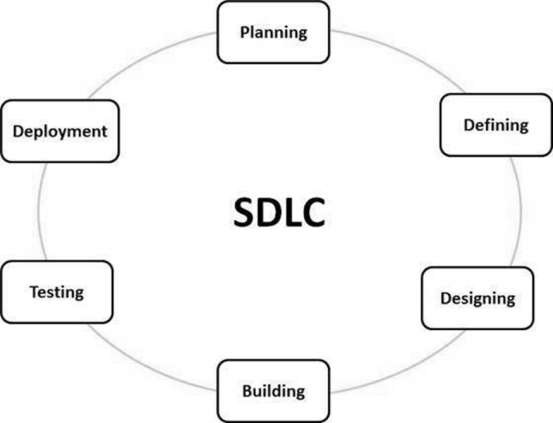
\includegraphics[width=10cm]{sdlc.jpg}
\caption{Der SDLC}
\end{center}
\end{figure}

\subsection{Ziele der klassischen bzw. statischen Softwareentwicklung}
Wie oben erwähnt, arbeiten klassische Softwareentwicklungsmodelle nach einem festen Plan (SDLC), welcher im Vorhinein festgelegt wird. Dieser Plan ist schwer veränderbar, d.h. Änderungen in den Anforderung müssen strikt überprüft werden, bevor sie implementiert werden.\\
Da jeder Arbeitsschritt klar festgelegt ist, ist es für die Entwickler einfach zu verstehen, was in dieser Phase der Entwicklung zu tun ist.\\
Damit dies funktioniert, ist es wichtig, dass die Anforderungen an das Produkt genau analysiert und festegehalten werden. Zudem ist eine sorgfältige Planung des Projektes von großer Wichtigkeit.\\
Damit Übersicht hergestellt werden kann, wird der Entwicklungsprozess sorgfältig dokumentiert und damit Fehler sofort festgestellt werden, wird die getane streng kontrolliert. \citep{stoica}

\subsection{Das Wasserfallmodell}
\subsubsection{Aufbau des Wasserfallmodells}
Das Wasserfallmodell funktioniert nach einem einfachen Prinzip: Eine Phase muss abgeschlossen sein, damit die nächste beginnen kann. Am Ende jeder Phase wird das Produkt überprüft, ob es die Anforderungen des Kunden erfüllt.\\
Beim Wasserfallmodell gibt es fünf Phasen, welche insgesamt dem SDLC ähneln.\\
In der ersten Phase werden die Anforderungen an das zu entwicklende Podukt zusammengetragen und analysiert.\\
Danach folgt das Designen des Systems in Phase zwei.\\
Darauf folgt Phase drei, bei welcher implementiert wird.\\
In Phase vier wird das Programm getestet.\\
In der finalen Phase fünf wird das System bereitgestellt und das System gegebenenfalls gewartet.\\
Alle Phasen werden genau dokumentiert um Übersicht herzustellen. \citep{stoica}\\
Aus diesem Aufbau des Modells ergeben sich sowohl Vorteile, als auch Nachteile.
\subsubsection{Vorteile des Wasserfallmodells}
Das Wasserfallmodell ist durch die Gliederung in Phasen, also einzelne Arbeitsschritte mit klaren Anforderungen, welche nacheinander ausgeführt werden, leicht zu verstehen und anzuwenden. Dies ist zum Beispiel von Vorteil, wenn es neues Teammitglied zum Team stößt.\\
Außerdem wird durch das stufenweise Vorgehen eine einfache Koordination gewährleistet. In jeder Phase muss ein bestimmtes, festgelegtes Zeil erreicht werden. Das ist einfach zu verstehen und durchzuführen. \citep{stoica}\\
Jedoch hat das Wasserfallmodell auch Nachteile.
\subsubsection{Nachteile des Wasserfallmodells}
Ein Nachteil des Wasserfallmodells ist es, dass es keine Flexibilität bei Anforderungsänderungen gibt, denn wenn diese eintreten, muss das Projekt neugeplant werden, wodurch von vorn begonnen werden muss.\\
Zudem gibt keine Prototypen des Produktes, bis alle Phasen durchlaufen wurden. Dadurch, weiß man bis zuletzt nicht, ob das Produkt den Anforderungen entspricht.\\
Außerdem ist es schwierig Probleme, welche beim Testen entstehen, zu beheben, da man dafür in die Systemdesignphase (zweite Phase) zurückkehren muss und somit damit nochmals alle anderen Phasen durchschreiten muss. \citep{stoica}

\newpage
\section{Die Agile Softwareentwicklung}
\subsection{Definition}
\begin{center}
\large{\glqq{} Agile Softwareentwicklung ist eine Entwicklungsmethode die schnell auf veränderte Anforderungen reagieren kann, da die Entwicklung in vielen kleinen und abgeschlossen Zyklen abläuft und eine erhöhte Kommunikation zwischen den Entwicklern stattfindet.\grqq{}}\footnote{aus:\url{https://www.gruenderszene.de/lexikon/begriffe/agile-softwareentwicklung?interstitial_click}} \\
\end{center}

\subsection{Leitsätze der Agilen Softwareentwicklung}
Die Leitsätze des Agiles Modells wurden von 11 Softwareentwicklern, unter der Führung von Kent Beck im \glqq{}Manifest für Agile Softwareentwicklung\grqq{} festgehalten. Es gibt vier wesentliche Leitsätze der Agilen Softwareentwicklung, welche sie von \\anderen Softwareentwicklungsmodellen abgrenzt:
\begin{itemize}
\item \glqq{}\textbf{Individuen und Interaktionen} mehr als Prozesse und Werkzeuge\grqq{} \cite{Beck2013} 
\item \glqq{}\textbf{Funktionierende Software} mehr als umfassende Dokumentation\grqq{} \cite{Beck2013} 
\item \glqq{}\textbf{Zusammenarbeit mit dem Kunden} mehr als umfassende Vertragsverhandlungen\grqq{} \cite{Beck2013} 
\item \glqq{}\textbf{Reagieren auf Veränderung} mehr als das Verfolgen eines Plans\grqq{} \cite{Beck2013} 
\end{itemize}
Angemerkt sei, dass die Entwickler des Agilen Modelles keinesfalls die Werte auf der rechten Seite als unwichtig betrachten, sondern die Werte auf der linken Seite als wichtiger im Prozess der Softwareentwicklung einschätzen.\\
Außerdem gibt es im Maifest eine Erweiterung der auf 12 Prinzipien, welche die oben genannten Prizipien näher erklären.\citep{Beck2013} 
\subsection{Prinzipien der Agilen Softwareentwicklung}
Ein Prinzip des Agilen Modells, dass die Menschen, welche an der Entwicklung beteiligt sind miteinander interagieren.\\\\
Im Agilen Modell ist es wichtig, dass die Entwickler dem Kunden oft ihr Zwischenergebnis schicken, um den Kunden zufrieden zu stellen.\\\\
Dazu gehört die enge Zusammenarbeit zwischen Fachexperten und die Softwareentwickler sollen währendes Projektes täglich miteinander arbeiten.\\\\
Die Entwickler sollen Kunden alle Anforderungsänderungen erfüllen, um dem Kunden einen Wettbewerbsvorteil verschaffen zu können.\\\\
Die Entwickler sollen dem Kunden funktionierende Software innerhalb eines bestimmten Zeitraumes (einige Wochen oder Monate, aber schnellstmöglich) liefern, damit der Kunde den Fortschritt sehen kann.\\\\
Zudem sollte auf motivierte Individuen vertraut werden. Es sollte ihnen die Ünterstützung gewährleistet werden, damit sie die Aufgabe erledigen können. Das Wichtigste ist das Vertrauen in die Individuen, dass sie die Aufgabe bewältigen können.\\\\
Um im Entwicklungsteam Informationen auszutauschen, ist es die beste Methode dies im Gespräch zu erledigen.\\\\
Die Entwickler, Auftraggeber und die Benutzer sollen ein gleichmäßiges Tempo auf unbegrenzte Zeit halten können, um nachhaltige Entwicklung zu fördern.\\\\
Ständige Priorität sollten technische Exzellenz und gutes Design haben, um Agilität zu fördern.\\\\
Einfachheut ist im Agilen Modell sehr wichtig und wird als \glqq{}die Kunst, die Menge nicht
getaner Arbeit zu maximieren\grqq{}\cite{Beck2013} verstanden.\\\\
Die besten Ergebnisse mit diesem Modell können durch selbstorganisierte Teams erzielt werden.\\\\
Das gesamte Team soll in regelmäßigen Abständen selbst reflektieren, wann es seine Effektivität verbessern kann. \citep{Beck2013}
\subsection{Paarprogrammieren}
Wie oben schon erwähnt, liegt der Fokus der Agilen Softwareentwicklung mehr Fokus auf den Entwicklern und deren Interaktion liegt, als auf den Werkzeugen, welche zur Programmierung verwendet werden. So kommt es, dass sich Methoden entwickelt haben, welche sich besonders gut für Agile Softwareentwicklung eignen.\\
Dazu wurde zum Beispiel die Methode des Paarprogrammierens (auch \glqq Pair Programming\grqq genannt) entwickelt. Dabei lösen zwei Entwickler eine Aufgabe an einem gemeinsamen Rechner.\\ 
Ein Programmierer ist dabei \glqq Driver\grqq{} und der andere \glqq Observer\grqq.
Der Driver hat die Kontrolle über das bzw. die Eingabegeräte. Das bedeutet, dass er den Code schreibt oder designt.\\
Der Observer hingegen \glqq überwacht\grqq{} den Driver. Seine Aufgabe sind es:
\begin{itemize}
\item auf Fehler aufmerksam zu machen, welche vom Driver begangen werden,
\item sich Alternativen auszudenken,
\item Resourcen zu finden, welche zur Entwicklung gebraucht werden oder
\item die Auswirkungen der aktuellen Arbeit einzuschätzen und im Gesamtkontext zu beachten.
\end{itemize}
Im Entwicklungsprozess werden die Rollen immer in regelmäßigen Zeitabständen getauscht. Wichtig zu beachten ist auch
Pair Programming ist sehr erfolgreich und wird daher oft in der Industrie eingesetzt.\\
Es verspricht eine höhere Qualität des Produktes mit geringerem Zeitaufwand. Dies wurde auch durch eine Studie der University of Utah belegt. Außerdem stellte sich heraus, dass sich die Programmierer beim Paarprogrammieren sicherer in ihrer Arbeit fühlen und mehr Spaß an der Arbeit haben, wenn sie zu zweit arbeiten anstatt allein.\\
Wenn allein programmiert wird, mündet es bei Drucksituationen (zum Beispiel: wenig Zeit) in unsauberem Arbeiten, wodurch die Qualität des Endproduktes sinkt. Wenn jedoch zu zweit programmiert wird, ist es leichter einen \glqq kühln Kopf\grqq zu bewahren, weil der Partner helfen kann, wenn es Komplikatonen geben sollte. \citep{pairprogramming}

\subsection{Ziele der Agilen Softwareentwicklung}
Aus den bereits aufgezeigten Prinzipien und Leitsätzen der Agilen Softwareentwicklung, kann man nun die Ziele  auch die damit verbunden Vorteile ableiten. \\
Schon die Prinzipien, die im \glqq{}Agilen Manifest\grqq{} niedergeschrieben wurden, geben Aufschluss darüber, was die Entwickler, welche dieses Modell der Softwareentwicklung nutzen, hinaus wollen.\\ Es wird Wert auf \glqq{}Individuen und Interaktionen, Funktionierende Software, Zusammenarbeit mit dem Kunden und das Reagieren auf Veränderung\grqq{} gelegt. Wie man erkennen kann, liegt der Fokus der Softwareentwicklung eher auf den Menschen, welche am Prozess der Entwicklung teilnehmen. So steht zum Beispiel der Kunde mit seine Wünschen im Vordergrund. Deshalb ist das Modell so ausgelegt, dass die Entwickler schnell auf Kundenwünsche bzw. -anregungen reagieren können.\\ Zudem werden auch die Entwickler mehr berücksichtigt und es werden auch spezielle Arbeitsmethoden angewendet (siehe oben)\\Außerdem empfinden die Nutzer der Agilen Softwareentwicklung die akribische Dokumentation des Schaffensprozesses als Behinderung der Arbeit und bauen lieber auf \glqq funktionierende Software\grqq. \\ 

\subsection{Extreme Programming}

\section{Vergleich von klassischer bzw. statischer und agiler Softwareentwicklung}



\section{Prozesse zur Erleichterung des Programmierens}
\subsection{Motivation}
Es gibt natürlich sehr viele verschiedene Varianten und Modelle eine Anwendung zu programmieren (siehe Kapitel 1), dabei sollten aber einige Dinge beachtet werden, um das Programm möglichst ansprechend für den Kunden und einfach prorammierbar zu gestalten. Außerdem kann so die Qualität des Programmes erheblich erhöht werden. 
\subsection{Vermeidung von Überflüssigem}
Hierbei gibt es im Wesebtlichen 3 Methoden zu nennen, mit welchen überflüssige Programmteile vermieden werden können.


\subsubsection{KISS}
Die Abkürzung \glqq KISS\grqq \ steht für \glqq Keep\grqq it simple, stupid", was übersetzt so viel heißt wie \glqq Mach es einfach, Dummkopf\grqq. \\
Der Name dieses Prinzips stammt von Kelly Johnson, einem englischen Ingenieur, der diesen Ausdruck im Jahr 1960 gesagt haben soll. \citep {goll_entwurfsprinzipien}  \\
Nach dem Prinzip KISS wird gehandelt, wenn das System möglichst einfach aufgebaut ist und wenig komplex ist. Durch erhöhte Komplexität, können spätere Änderungen und Erweiterungen nicht durchgeführt werden, ohne "die Stabiblität des Systems zu gefährden"\  \cite{goll_entwurfsprinzipien}.\\\\
Da KISS Einfachheit fordert, ergeben sich viele Vorteile. \\
Natürlich ist es einfacher ein einfaches, weniger komplexes System  \glqq zu verstehen, zu bauen, zu testen, zu ändern und zu warten\grqq\ \cite{goll_entwurfsprinzipien}.\\
Außerdem können weniger Fehler im System auftreten, da es auch weniger Komponenten gibt, welche eben diese aufweisen können.\\
Ein Nachteil von KISS ist es, dass einfache Systeme, meist schwieriger zu programmieren sind, da komplexe Lösungen meist einfacher zu implementieren sind.\\
Zudem sollte beachtet werden, dass KISS zwar beinhaltet, einfache Systeme zu bauen, jedoch keine monolithischen, welche ungegliedert sind und somit die Arbeit erschweren. \citep{goll_entwurfsprinzipien}
\subsubsection{YAGNI}
\glqq YAGNI\grqq{} kommt aus dem Englischen und steht für \glqq You aren't gonna need it\grqq, was übersetzt so viel bedeutet, wie \glqq Du wirst es nicht brauchen.\grqq\\
Diese Technik wurde maßgeblich von Ron Jeffries et al.\footnote[1]{Ron Jeffries war einer der Initiatoren der agilen Softwareentwicklung und hat u. A. das \glqq Agile Manifest\grqq mitentwickelt.} geprägt und wird deshalb auch oft mit der agilen Softwareentwicklung in Verbindung gebracht (siehe Kapitel 1.2) \citep{Jeffries}\\
Generell soll mit diesem Prinzip \glqq Over-Engineering\grqq \  \cite{goll_entwurfsprinzipien} und eine \glqq spekulative Generalisierung\grqq\  \cite{goll_entwurfsprinzipien} vom Entwickler vermieden werden.\\
Als Over-Engineering wird die Entwicklung eines Produktes höherer Qualität und größerem Aufwand, als der Kunde gefordert hat, bezeichnet. Somit wird meist der Preisrahmen des Kunden überschritten.\\
Spekulative Generalisierung bedeutet, dass der Entwickler Abstraktionen einführt, die er denkt, noch gebrauchen zu können, obwohl diese meist später nicht mehr benötigt werden. \glqq Generalisierungen verzögern [außerdem] das ursprüngliche Projekt, erschweren die Ausbaubarkeit und kosten Geld\grqq \ \cite{goll_entwurfsprinzipien}. Auch Generalisierungen sollten vom Kunden gewünscht und bezahlt werden. Sonst ist es empfehlenswert diese wegzulassen.\\\\
Durch YAGNI ergeben sich viele Vorteile für den Entwickler und auch für den Kunden.\\
Zum Einen ist der geschriebene Code einfach weiterentwickelbar, weil er im besten Fall wenig komplex und übersichtlich ist und außerdem nicht durch überflüssige Funktionalität behindert wird.\\
Durch generalisierte Feautures im Produkt können unnötige Einschränkungen auftreten, welche sich aber durch YAGNI verhindern lassen.\\
Zudem hat der Entwickler mehr Zeit sich auf die geforderten Funktionen des Kunden zu konzentrieren, weil er die Zeit, die er durch verzichtbare Generalisierung vergeudet, sinvoll nutzen kann.\\\\
Jedoch kann es bei einer falschen Anwendung von YAGNI auch zu einem Problem kommen. Denn wenn sich der Entwickler nur auf die Anwendungsfunktionen des Programmes fokussiert, kann es dazu kommen, dass die Weiterentwickelbarkeit des Programmes nicht berücksichtigt wird. Das ist falsch, denn auch wenn der Kunde die Infrastruktur des Produktes nicht kennt, sollte auch diese, nicht übertrieben, beachtet werden. \citep{goll_entwurfsprinzipien}

\subsubsection{DRY}
\glqq DRY\grqq \ kommt aus dem Englischen und steht für \glqq Don't repeat yourself\grqq, was auf Deutsch übersetzt soviel wie \glqq Wiederhole dich nicht\grqq\ bedeutet. \\
Diese Abkürzung stammt von Andrew Hunt und David Thomas aus ihrem Buch \glqq Der Pragmatische Programmierer\grqq\  \citep{hunt} wurde aber keineswegs von diesen Personen erfunden. Davor war es als \glqq Single-Source-Prinzip\grqq\  bekannt. \citep{goll_entwurfsprinzipien}\\
Beim Programmieren können Redundanzen entstehen. Redundanzen oder auch Replikate sind Programmteile, welche identisch sind. Diese treten zum Beispiel durch Unaufmerksamkeiten, Zeitnot und fehlender Absprache zwischen den Teammitgliedern auf.\\
Diese Redundanzen sollen mit dem DRY-Prinzip verhindert werden, denn Replikate bringen oftmal Schwierigkeiten, wie zum Beispiel das Erzeugen von inkonsistenten Informationen bei Aktualisierung des Programmes, mit sich. \\
Deshalb sollten in einem Programm, in welchem dieses Prinzip beachtet wurde,  alle Informationen des Projektes lediglich einmal vorkommen.
\\\\Durch DRY werden \glqq Aktualisierungsprobleme vermieden (siehe oben) und dadurch die Komplexität verringert\grqq\ \cite{goll_entwurfsprinzipien}.\\
Außerdem wird der Code durch DRY besser lesbar, weil schlichtweg weniger Code vorhanden ist.\\
Jedoch kann es auch passieren, dass bei manchen Programmen Redundanzen vorhanden sein müssen, welche dann fälschlicherweise durch DRY entfernt wurden.
\subsubsection{Zusammenfassung}
Die drei vorgestellten Methoden nehmen keinen Einfluss auf die Struktur bzw. Architektur des Programmes, sondern sollten vom Entwickler beim Programmieren beachtet werden, damit die Programme besser verständlich und stabiler werden und zudem wechselseitige Abhängigkeiten abgeschwächt werden können. Somit kann die Komplexität des Produktes reduziert werden. \citep{goll_entwurfsprinzipien}\\
Im nachfolgenden Abschnitt werden die Prinzipien zur Verringerung der Komplexität vorgestellt, welche auf Systemebene wirken.

\subsection{Prozesse auf Systemebene}
\subsubsection{Divide And Conquer}
\glqq Divide and conquer\grqq oder zu Deutsch \glqq \ Teile und Herrsche\grqq bezeichnet ein viel in der Informatik eingesetztes Prinzip.\\
 \glqq Teile und Herrsche\grqq \ funktioniert, indem ein großes Problem rekursiv zerlegt wird, so dass viele kleine Teilprobleme enstehen, welche dann einfacher gelöst werden können. Die Teilprobleme lassen sich dann am Ende zusammensetzten und bilden somit das Programm.\\
Somit kann man zum Beispiel Algorithmen entwerfen und zum Beispiel ein Programm in viele Module zerlegen.\\
Ziel von \glqq Divide And Conquer\grqq\  ist es, ein schweres, komlexes Ausgangsproblem von oben nach unten \glqq in kleinere, möglichst unabhängige Teilprobleme\grqq \ \cite{goll_entwurfsprinzipien} zu zerlgen, um diese dann möglichst einfach zu lösen.\\
Auch \glqq Teile und Herrsche\grqq\  bringt Vorteile, als auch Nachteile, mit sich.\\
So wird aus einem ursprünglich sehr komlexen Problem, ein Einfaches gemacht, wodurch die Komplexität verloren geht.\\
Außerdem ist es ein Vorteil, dass viele kleine Probleme gelöst werden, denn wenn bei diesen ein Fehler auftritt, kann dieser leicht behoben werden und es entstehen keine großen Probleme.\\
Jedoch ist der Top-Down-Ansatz \footnote[2]{Zerlegung des Problems von oben nach unten} nicht immer passend. Das bedeutet, \glqq wenn eine untere Ebene, beispielsweise Bibliotheken, vorgegeben sind: Dann muss die Zerlegung so erfolgen,dass man diese Ebene auch "trifft".\grqq \ \cite{goll_entwurfsprinzipien}

\subsubsection{Design to Test}
Ein wichtiger Teil des Programmiers ist auch das Testen (siehe Kapitel 1.2). Jedoch kommt dieser Entwicklungsabschnitt meist zu kurz, da die Performance des Produktes meht  im Vordergrund steht. Somit ist das Produkt am Ende, dass sich der Gesamttest ungenügend automatisieren lässt. Somit steigen auch die Kosten sowohl beim Gesamtsystemtest, als auch bei der Wartung.\\
Ein Gesamtsystemtest ist leichter durchzuführen, wenn alle Komponenten einzeln (siehe \glqq Divide And Conquer\grqq) getestet werden können. Dies stellt auch das Ziel des Prinzips \glqq Design to Test\grqq dar. Das bedeutet, dass ein Programmteil so entworfen werden sollte, dass es einfach zu testen ist. Wenn dies nicht der Fall ist sollte der Programmteil verworfen werden und eine gut testbare Lösung gefunden werden.\\
Die gute Testbarkeit eines Programmes bringt Vorteile mit sich.\\
Zum Beispiel können alle Tests automatisiert ablaufen.\\
Außerdem können alle Programmteile besser getestet werden, dadurch senken sich die Kosten für das Testen.\\
Jedoch ist es ein Nachteil, wenn erst nach dem Entwurf feststellt wird, dass dieser schlecht testbar ist, da somit die Entwicklungskosten durch den Neuentwurf ansteigen. Deshalb sollte auch beim Planen, sowie bei allen Schritten der Produktentwicklung, auch die Testbarkeit im Vordergrund stehen, so dass hohe Kosten durch Neuentwürfe vermieden werden können. \citep{goll_entwurfsprinzipien}

\subsection{Bildquellen}
\url{http://www.tutorialspoint.com/sdlc/sdlc_overview.htm}

\newpage
\bibliography{bellBib}


\end{document}